% !TeX root = RJwrapper.tex
\title{\pkg{pdynmc}: A Package for Estimating Linear Dynamic Panel Data Models Based on Nonlinear Moment Conditions}
\author{by Markus Fritsch, Andrew Adrian Yu Pua and Joachim Schnurbus}

\maketitle




\abstract{
This paper introduces \CRANpkg{pdynmc}, an R package that provides users sufficient flexibility and precise control over the estimation and inference in linear dynamic panel data models. The package primarily allows for the inclusion of nonlinear moment conditions and the use of iterated GMM; additionally, visualizations for data structure and estimation results are provided. The current implementation reflects recent developments in literature, uses sensible argument defaults, and aligns commercial and noncommercial estimation commands.
Since the understanding of the model assumptions is vital for setting up plausible estimation routines, we provide a broad introduction of linear dynamic panel data models directed towards practitioners before concisely describing the functionality available in \pkg{pdynmc} regarding instrument type, covariate type, estimation methodology, and general configuration. We then demonstrate the functionality  by revisiting the popular firm-level dataset of \citet[]{AreBon1991}.
}









\section{Introduction}
This paper introduces the contributed package \pkg{pdynmc} \citep{FriPuaSchn2020} -- a unified framework for estimating linear dynamic panel data models based on linear and nonlinear moment conditions \citep{AhnSch1995}. Our implementation of the commands in \pkg{pdynmc} allows the user to exert precise control over the available functionality, reflects recent developments in literature, uses sensible argument defaults, aligns commercial and noncommercial estimation commands, and provides visualizations of data structure and estimation results. Additionally, this paper provides a concise introduction into linear dynamic panel data models directed towards the practitioner, describes the functionality available in \pkg{pdynmc}, and walks the reader through estimation of linear dynamic panel data models by replicating the analysis in \cite{AreBon1991}.

Practitioners have a variety of recent packages that enable linear dynamic panel data modeling meant for a fixed number of time periods. In particular, contributed R packages such as \CRANpkg{OrthoPanels} \citep{pickup2017orthopanels}, \CRANpkg{plm} \citep{CroMil2019plm}, and \CRANpkg{panelvar} \citep{SigFer2019panelvar} have considerably enlarged the set of noncommercial routines available. All of these packages implement some default routines for estimating common parameters in linear dynamic panel data models. \CRANpkg{OrthoPanels} implements a likelihood-based orthogonal reparameterization procedure for first-order autoregressive linear panel data models with strictly exogenous covariates. \CRANpkg{plm} implements one-step and two-step GMM-based procedures for $p$th-order autoregressive linear panel data models. \CRANpkg{panelvar} implements iterated  (or ``$m$-step'', compare \citealp{SigFer2019panelvar}) GMM  procedures for $p$th-order vector autoregressive linear panel data models. For the latter two packages, linear moment conditions are used to identify common parameters.

Additional functionality of our contributed package \pkg{pdynmc} includes nonlinear moment conditions which are generally not available across standard GMM estimation routines. To the best of our knowledge, there is currently only the xtdpdgmm-implementation provided by \citep{Kri2019} for the commercial statistical software Stata \citep{Sta2015}. The current implementation in Stata restricts accessibility to the routine as it requires a recent Stata version (version 13 or higher).
Another key estimation option provided by \pkg{pdynmc} is iterated GMM. \citet{HansenLee2020} recently outlined the merits of the technique and developed the theory under potential misspecification of moment conditions.
The availability of iterated GMM for dynamic panels may help to apply the results found in, for example, \citet{HWANG2018381}. Visualizations of the estimation results of iterated GMM are also included.

The structure of the paper is as follows. Section \hyperref[sec:ldpdm]{Framework and methodology} briefly sketches the linear dynamic panel data model, states underlying assumptions frequently used in literature, and describes moment conditions arising from different sets of model assumptions. Section \hyperref[Sec:R]{R implementation} covers details on the arguments of the model fitting function \code{pdynmc} and connects the description with the estimation methodology.
Section \hyperref[sec:example]{Empirical example} illustrates the estimation of linear dynamic panel data models with \pkg{pdynmc} for the dataset of \citet{AreBon1991}, while Section \hyperref[sec:conclusion]{Conclusion} concludes.















\section{Framework and methodology}\label{sec:ldpdm}
Linear dynamic panel data models account for dynamics and unobserved individual-specific heterogeneity. Due to the presence of lagged dependent variables, applying ordinary least squares including individual-specific dummy variables is inconsistent \citep[see, e.g.,][]{Hsi2014}.
A suitable alternative for obtaining parameter estimates of linear dynamic panel data models is deriving moment conditions (or population orthogonality conditions) from the model assumptions. The moment conditions may be linear \citep{AndHsi1982,HolNewRos1988,AreBov1995} or nonlinear \citep{AhnSch1995} in parameters and determine the natural instruments available for estimation. Usually, the number of moment conditions exceeds the number of parameters, and the moment conditions need to be aggregated appropriately. This can be achieved by the generalized method of moments (GMM), where weighted linear combinations of moment conditions are employed to obtain parameter estimates.

Theoretical results and evidence from Monte Carlo simulations in the literature suggest that incorporating nonlinear (quadratic) moment conditions proposed by \citet{AhnSch1995} is valuable for identification. For example, when the lag parameter exhibits high persistence, linear moment conditions fail to identify the model parameters, while quadratic moment conditions can still provide identification \citep{BunKle2014,BunSar2015,GorHanXue2016,PuaFriSch2019a,PuaFriSch2019b}.
Note that the quadratic moment conditions are immediate by-products of imposing
standard assumptions, which are the basis of the \cite{AreBon1991} estimator -- the most popular default routine in dynamic panel data estimation.

Since the moment conditions employed in GMM estimation of linear dynamic panel data models are derived from model assumptions, a basic understanding of these assumptions is vital for setting up a plausible estimation routine. We briefly review the assumptions implied when using particular moment conditions in the estimation below and add to the exposition in the \pkg{plm} vignette \citep{CroMil2019plm}, where the function \code{pgmm} is used to estimate linear dynamic panel data models. For further reading on the methodology, we suggest \citet{Fri2019}.


\subsection{Linear dynamic panel data model}
For a given dataset with cross-section dimension $n$ and time series dimension $T$, consider a linear dynamic panel data model of the form:
\begin{align}
y_{i, t} & = \alpha y_{i, t - 1} + \beta x_{i, t} + u_{i,t}, \quad i = 1, \dots, n;\ t = 2, \dots, T,\label{EQ00-1:lin-dyn-pdm} \\
u_{i,t} & = \eta_{i} + \varepsilon_{i, t}. \label{EQ00-2:lin-dyn-pdm}
\end{align}
Variables $y_{i,t}$ and $y_{i,t-1}$ denote the dependent variable and its lag, $\alpha$ is the lag parameter, and $x_{i,t}$ is a single covariate with corresponding slope coefficient $\beta$. The second equation separates the composite error term $u_{i,t}$ into an unobserved individual-specific effect $\eta_i$ and an idiosyncratic remainder component $\varepsilon_{i,t}$.

Combining Equations (\ref{EQ00-1:lin-dyn-pdm}) and (\ref{EQ00-2:lin-dyn-pdm}) yields the single equation form:
\begin{align} \label{EQ01:lin-dyn-pdm}
y_{i, t} & = \alpha y_{i, t - 1} + \beta x_{i, t} + \eta_{i} + \varepsilon_{i, t}.
\end{align}

We only include one lag of the dependent variable, one covariate, and omit unobserved time-specific effects in this section for simplicity of exposition and notational convenience. Extending the representation is straightforward, and \pkg{pdynmc} can also accommodate AR($p$) models and time effects. The initial time period is denoted by $t=1$.

The unobserved individual-specific effects $\eta_i$ may be eliminated from Equation (\ref{EQ01:lin-dyn-pdm}) by taking first differences:
\begin{align} \label{EQ03:FDlin-dyn-pdm}
\Delta y_{i, t} = \alpha \Delta y_{i, t - 1} + \beta \Delta x_{i, t} + \Delta \varepsilon_{i, t}.
\end{align}
Since the first difference of the lagged dependent variable $\Delta y_{i,t-1} = y_{i,t-1} - y_{i,t-2}$ and the first difference of the idiosyncratic remainder component $\Delta \varepsilon_{i,t} = \varepsilon_{i,t} - \varepsilon_{i,t-1}$ are not orthogonal, ordinary least squares estimation of Equation (\ref{EQ03:FDlin-dyn-pdm}) is inconsistent. Linear dynamic panel data models are usually estimated by GMM, where corresponding moment conditions are derived from model assumptions.




\subsection{Standard assumptions and associated moment conditions}\label{sec:StdAssumpt}
Researchers have focused on the following standard assumptions, henceforth StA, \citep[see][]{AhnSch1995}:
\begin{align} \label{EQ02:StdAssumpt}
& \text{The data are independently distributed across} \ i, \\
& E(\eta_i) = 0, \quad i=1,...,n, \nonumber \\
& E(\varepsilon_{i,t}) = 0, \quad i=1,...,n,\ t=2,...,T, \nonumber \\
& E(\varepsilon_{i,t} \cdot \eta_i) = 0, \quad i=1,...,n,\ t=2,...,T, \nonumber \\
& E(\varepsilon_{i,t} \cdot \varepsilon_{i,s}) = 0, \quad i=1,...,n,\ t \neq s, \nonumber \\
& E(y_{i,1} \cdot \varepsilon_{i,t}) = 0, \quad i=1,...,n,\ t=2,...,T, \nonumber \\
& n \rightarrow \infty, \ \text{while}\ T \  \text{is fixed, such that}\ \frac{T}{n} \rightarrow 0. \nonumber
\end{align}
We assume that StA hold for the rest of this paper.

Under StA, \citet{HolNewRos1988} (henceforth \strong{HNR}) propose the moment conditions:
\begin{align}\label{EQ04:HNR-MC-linear}
E(y_{i,s} \cdot \Delta u_{i,t}) = 0, \qquad t = 3,\dots,T;\ s = 1,\dots,t - 2.
\end{align}
Equation (\ref{EQ04:HNR-MC-linear}) provides $0.5(T-1)(T-2)$ moment conditions.
Equivalent moment conditions can be derived from the covariate $x_{i,t}$ -- depending on its correlation with the idiosyncratic remainder component $\varepsilon_{i,t}$. Endogenous, predetermined, and (strictly) exogenous covariates provide the following linear moment conditions, respectively:
\begin{align} \label{EQ06:HNR-MC-linear-x_it}
E(x_{i,s} \cdot \Delta u_{i,t}) = 0, \qquad t = 3,\dots,T, \qquad &\text{where}& \\
s = 1,\dots,t - 2, \qquad &\text{for} \qquad \text{endogenous}\ x, \nonumber \\
s = 1,\dots,t - 1, \qquad &\text{for} \qquad \text{predetermined}\ x, \nonumber \\
s = 1,\dots,T,     \qquad &\text{for} \qquad \text{strictly exogenous}\ x. \nonumber
\end{align}
After solving Equation (\ref{EQ00-1:lin-dyn-pdm}) for $u_{i,t}$ and inserting this as $\Delta u_{i,t} = u_{i, t} - u_{i, t - 1}$, it is apparent that the HNR moment conditions are linear in parameters ($\alpha$ and $\beta$). In literature, the HNR moment conditions also appear as ``moment conditions with instruments in levels'' (w.r.t.\ $y_{i,s}, x_{i, s}$) and ``moment conditions from equations in differences'' (w.r.t.\ $\Delta u_{i, t}$).





\citet{AhnSch1995} (henceforth \strong{AS}) have shown that under StA the following $T-3$ additional moment conditions hold:
\begin{align}\label{EQ05:AS-MC-nonlinear}
E(u_{i,T} \cdot \Delta u_{i,t-1}) = 0, \qquad t = 4,\dots,T.
\end{align}
These moment conditions are nonlinear in parameters (quadratic in $\alpha$ and $\beta$).











\subsection{Extended assumptions and associated moment conditions} \label{sec:ExtAssumpt}
Another set of moment conditions, beyond those implied by StA, that is popular in theoretical and applied research is derived from the assumption:
\begin{equation} \label{EQ07:CCE}
E(\Delta y_{i,t} \cdot \eta_i) = 0, \quad i=1,\dots,n.
\end{equation}
This expression requires that the dependent variable and the unobserved individual-specific effects are constantly correlated over time for each individual and has thus been called ``constant correlated effects'' \citep[][]{BunSar2015}. This assumption is also called ``effect stationarity'' \citep[][]{Kiv2007a} or ``mean stationarity'' \citep[][]{Are2003}.

From this assumption, \citet{AreBov1995} derive $T-2$ additional moment conditions (henceforth \strong{ABov}):
\begin{align} \label{EQ08:AB-MC-linear_yit}
E(\Delta y_{i,t-1} \cdot u_{i,t}) = 0, \quad t=3,\dots,T.
\end{align}
By rewriting these moment conditions, it can be shown that the ABov moment conditions encompass the nonlinear AS moment conditions \citep[for a derivation see][]{Fri2019}.

Depending on the assumptions about $x_{i,t}$, additional ABov moment conditions can be derived:
\begin{align*}
E(\Delta x_{i,v} \cdot u_{i,t}) = 0, \qquad & \text{where} \\
& v = t-1;\ t=3, \dots T, \quad\text{for} \quad x \ \  \text{endogenous}, \\
& v = t;\ t=2,\dots,T, \quad \text{for} \quad x \ \ \text{strictly exogenous} \quad \text{or} \quad x \ \ \text{predetermined}.
\end{align*}


Deviations from the assumption are required to be unsystematic over both the cross-section and the time series dimension \citep[see Section 6.5 in][which also provides an empirically relevant example]{Are2003}.
Employing the constant correlated effects assumption implicitly constrains the relationship between $\Delta x_{i,t}$ and $\eta_i$ \citep[see][]{BluBonWin2001}. If the statistician is not willing to impose this restriction, nonlinear AS moment conditions can be used instead.





















\section{R implementation}\label{Sec:R}
Similar to function \code{pgmm} in the package \CRANpkg{plm}, \pkg{pdynmc} provides one-step and two-step closed-form GMM estimators and standard specification testing such as overidentifying restrictions tests, serial correlation tests, and Wald tests. These features are shared by other packages implemented in Gauss, Ox \citep{DooAreBon2012dpd}, R, and Stata. We provide options to match results from other statistical software estimation routines. In contrast to \pkg{OrthoPanels} and \pkg{plm}, \pkg{pdynmc} does not include a formula interface to allow the user to exert full control over all functionality.





\subsection{GMM estimation, inference, and testing}
We provide one-step, two-step, and iterated estimation for the coefficients.
The weighting matrix of the moment conditions plays a prominent role in estimation \citep{AreBon1991,BluBonWin2001,Kri2019}. An optimal weighting matrix is proportional to the inverse of the covariance matrix of the moment conditions \citep[see, e.g.,][]{Are2003}.
The default weighting matrix used in \pkg{pdynmc} is based on the proposal of \citet{AreBon1991}. For details on available alternatives, see the documentation of \pkg{pdynmc} and the corresponding package vignette \citep{FriPuaSchn2020}.

Details on the computation of asymptotic one- and two-step standard errors can be found in \citet{DooAreBon2012dpd}.
As asymptotic two-step GMM standard errors for the estimated coefficients exhibit a downward bias in small samples, they can be substantially lower than one-step GMM standard errors \citep[see, e.g.,][]{AreBon1991}. \citet{Win2005} relates the bias to the dependence of the two-step weighting matrix on one-step parameter estimates and proposes an analytic correction of two-step standard errors.
Robust and non-robust versions of the standard errors are available.

Coefficient estimates and standard errors from one- and two-step GMM estimation can be misleading. An example of high practical relevance is when the estimated model is a reasonable approximation instead of the true functional relationship \citep{HansenLee2020, HwangKangLee2020}: This may render some of the moment conditions invalid. \citet{HansenLee2020} highlight the arbitrariness of the initial weighting matrix and note that iterated GMM provides a remedy. Across iterations, the weighting matrix is updated based on the residuals of the previous estimation step \citep[for more details, see][p. 4--6]{HansenLee2020}. Iterated GMM is used as a default in \pkg{pdynmc}.


We implement the following tests:
\begin{itemize}
\item The serial correlation test of \citet{Are2003}.
\item The overidentifying restrictions test of \citet{Han1982large}, called ``J-test''.
\item A Wald test of joint significance of (i) coefficients of lagged-dependent variable(s) and covariates; (ii) time dummy coefficients; (iii) both, (i) and (ii).
\end{itemize}




When nonlinear moment conditions are used in GMM estimation, nonlinear optimization techniques are required to obtain coefficient estimates. By default, GMM estimation by \pkg{pdynmc} is based on numerical optimization.
For the optimization procedure, we rely on R-package \CRANpkg{optimx} \citep{NasVar2011,Nas2014}. All optimization routines implemented in \pkg{optimx} are available in \pkg{pdynmc}. Based on our experience, we recommend using the Variable Metric method \citep{Fle1970new,Nas1990compact,Nas2020} in the estimation of linear dynamic panel data models.
The technique is labeled \code{BFGS} in \pkg{optimx} and serves as the default procedure in \pkg{pdynmc}.


















\subsection{Function arguments explained}
In package \pkg{pdynmc}, the eponymous function is intended for model fitting. The most important function arguments for applied work are summarized in Table \ref{Tab:arguments}.
\begin{table}[hptb]
\begin{tabular}{lp{11cm}}
    \toprule
Argument        &   Description \\
    \midrule
\code{dat}                  & Dataset with rows (i.e., observations) and columns (i.e., variables). \\
\code{varname.i}            & Cross-section identifier (column name). \\
\code{varname.t}            & Time series identifier (column name). \\
    \midrule
\code{use.mc.diff}          & Use moment conditions from Equation (\ref{EQ04:HNR-MC-linear}) (i.e., equations in differences, instruments in levels).   \\
\code{use.mc.lev}           & Use moment conditions from Equation (\ref{EQ08:AB-MC-linear_yit}) (i.e., equations in levels, instruments in differences).  \\
\code{use.mc.nonlin}        & Use nonlinear (quadratic) moment conditions from Equation (\ref{EQ05:AS-MC-nonlinear}).  \\
\code{use.mc.nonlinAS}      & If turned to \code{FALSE}, the nonlinear moment conditions are used in a modified version (that is also valid under StA), where $T$ in Equation (\ref{EQ05:AS-MC-nonlinear}) is replaced by $t$. \\
    \midrule
\code{include.y}            & Derive instruments from lags of dependent variable. \\
\code{varname.y}            & Name of dependent variable in dataset.  \\
\code{lagTerms.y}           & Number of lags of dependent variable.  \\
\code{maxLags.y}            & Maximum number of lags of dependent variable from which to derive instruments.  \\
    \midrule
\code{include.x}            & Derive instruments from covariates.  \\
\code{varname.reg.end}      & Name(s) of covariate(s) to be treated as endogenous (replace suffix \code{end} by \code{pre} for predetermined; by \code{ex} for exogenous covariates). \\
\code{lagTerms.reg.end}     & Number of lags of endogenous covariate(s) (also for \code{pre} or \code{ex}).   \\
\code{maxLags.reg.end}      & Maximum number of lags of endogenous covariate(s) used to derive instruments (also for \code{pre} or \code{ex}).  \\
    \midrule
\code{fur.con}              & Include further control variables (i.e., covariates that are not used for deriving instruments).    \\
\code{fur.con.diff}         & Logical variable indicating whether to include further control variables in equations in differences.  \\
\code{fur.con.lev}          & Logical variable indicating whether to include further control variables in equations in levels.  \\
\code{varname.reg.fur}      & Name(s) of covariate(s) in dataset to be treated as further controls.  \\
\code{lagTerms.reg.fur}     & Number of lags of further controls.  \\
    \midrule
\code{include.dum}          & Include time dummies. Note: Can be constructed from multiple variables. \\
\code{dum.diff}             & Include time dummies in equations in first differences.  \\
\code{dum.lev}              & Include time dummies in equations in levels.  \\
\code{varname.dum}          & Variable name(s) for creating time dummies (can be different from \code{varname.t}). \\
    \midrule
\code{w.mat}                & Type of initial weighting matrix to be used, \code{iid.err} (as proposed by \citet{AreBon1991}), \code{identity}, or \code{zero.cov}.  \\
\code{std.err}              & Type of standard errors to be used, either bias-corrected (\code{corrected}) according to \citet{Win2005} or not (\code{unadjusted}). \\
\code{estimation}           & Type of estimation, \code{onestep}, \code{twostep}, or \code{iterative}.  \\
    \bottomrule
\end{tabular}
\centering\caption{Most-used arguments of function \code{pdynmc}.} \label{Tab:arguments}
\end{table}




Besides the arguments described in Table \ref{Tab:arguments}, various further configuration options exist for function \code{pdynmc}.
The function allows for the inclusion of further covariates which are only used as instruments (i.e., covariates from which moment conditions are derived, but for which no parameters are estimated; compare arguments \code{include.x.instr} and
\code{varname.reg.instr}) as well as the opposite, covariates which are instrumented (i.e., covariates for which parameters are estimated, but from which no moment conditions are derived; compare arguments \code{include.x.toInstr} and \code{varname.reg.toInstr}).

Further, thresholds for collinearity checks can be adjusted via \code{col\_tol}. The total number of instruments above which a generalized inverse is used to invert the weighting matrix can be specified by \code{inst.thresh}.

When only linear moment conditions are used, a closed-form solution exists for the estimator, and nonlinear optimization can be turned off (by \code{opt.meth = "none"}).
Package \pkg{optimx} is employed for nonlinear optimization and argument \code{hessian} controls whether the Hessian matrix is approximated in estimation. All other control arguments for \pkg{optimx} can be provided in a list via \code{optCtrl}.
Starting values for initializing nonlinear optimization are drawn from the uniform distribution in the interval [-1, 1] via \code{start.val.lo = -1} and \code{start.val.hi = 1}; a seed (\code{seed.input = 42}) ensures reproducibility (limits and seed can be adjusted). Alternatively, specific starting values can be provided via argument \code{start.val} (note that \code{custom.start.val} has to be set to \code{TRUE}).

For iterated estimation, termination criteria can be set via \code{max.iter} (maximum number of iterations) and \code{iter.tol} (tolerance for determining convergence).

The Stata packages xtabond2 \citep{Roo2018xtabond2} and xtdpdgmm have somewhat different usage and weighting of moment conditions.
If HNR and ABov moment conditions are available for estimation, some of the ABov moment conditions are redundant \citep[see][for a derivation]{Fri2019}. While the Stata routines fully expand the linear ABov moment conditions when setting up the instrument matrix (including the redundant moment conditions), \pkg{pdynmc} omits the redundant moment conditions.
The \pkg{pdynmc} arguments \code{inst.stata} and \code{w.mat.stata} are included to allow for conformity to Stata and to reproduce estimation results.















\section{Empirical example}\label{sec:example}
The functionality of \pkg{pdynmc} is illustrated by replicating \citet{AreBon1991} in a wide sense as we incorporate linear ABov and nonlinear AS moment conditions into the analysis; we also draw comparisons between \pkg{pdynmc}, the \code{pgmm} \citep{CroEtAl2020plm} function in R-package \pkg{plm}, and Stata implementations xtabond2 and xtdpdgmm \citep{Kri2019}.

\citet{AreBon1991} employ an unbalanced panel of $n=140$ firms located in the UK. The dataset spans $T=9$ time periods and is available from R package \pkg{plm}.
\citet{AreBon1991} investigate employment equations and consider the dynamic specification:
\begin{align} \label{EQ18:ABEstimation}
n_{i,t} =& \alpha_1 n_{i,t-1} + \alpha_2 n_{i,t-2} + \\
&\beta_1 w_{i,t} + \beta_2 w_{i,t-1} + \beta_3 k_{i,t} + \beta_4 k_{i,t-1} + \beta_5 k_{i,t-2} + \beta_6 ys_{i,t} + \beta_7 ys_{i,t-1} + \beta_8 ys_{i,t-2} + \nonumber \\
& \gamma_3 d_3 + \dots + \gamma_T d_T + \eta_i + \varepsilon_{i,t}, \qquad i = 1,...,n;\ t = 3,...,T, \nonumber
\end{align}
where $i$ denotes the firm, and $t$ is the time series dimension. The natural logarithm of employment ($n$) is explained by its first two lags and the further covariates natural logarithm of wage ($w$), the natural logarithm of capital ($k$), the natural logarithm of output ($ys$), and their lags of order up to one (for $w$) or two (for $k$ and $ys$). Variables $d_3, \dots, d_T$ are time dummies with corresponding coefficients $\gamma_3, \dots, \gamma_T$; unobserved individual-specific effects are represented by $\eta$, and $\varepsilon$ is an idiosyncratic remainder component.

We load the dataset and compute logarithms of the four mentioned variables via:
\begin{example}
data(EmplUK, package = "plm")
dat             <- EmplUK
dat[,c(4:7)]    <- log(dat[,c(4:7)])
names(dat)[4:7] <- c("n", "w", "k", "ys")
\end{example}


As GMM estimation with linear and/or nonlinear moment conditions in \pkg{pdynmc} allows for arbitrary unbalancedness, we included the functions \code{data.info} and \code{strucUPD.plot} to provide an overview of the panel data structure. Both functions require the column name of cross-section (\code{i.name}) and time series identifier (\code{t.name}).
Using \code{data.info(dat, i.name = "firm", t.name = "year")} yields:
\begin{example}
Unbalanced panel dataset with 1031 rows and the following time period frequencies:
1976 1977 1978 1979 1980 1981 1982 1983 1984
  80  138  140  140  140  140  140   78   35
\end{example}
The command \code{strucUPD.plot(dat, i.name = "firm", t.name = "year")} gives the visual representation of the panel data structure shown in Figure \ref{fig:strucUPDplot}.
\begin{figure}[ht]
  \centering
  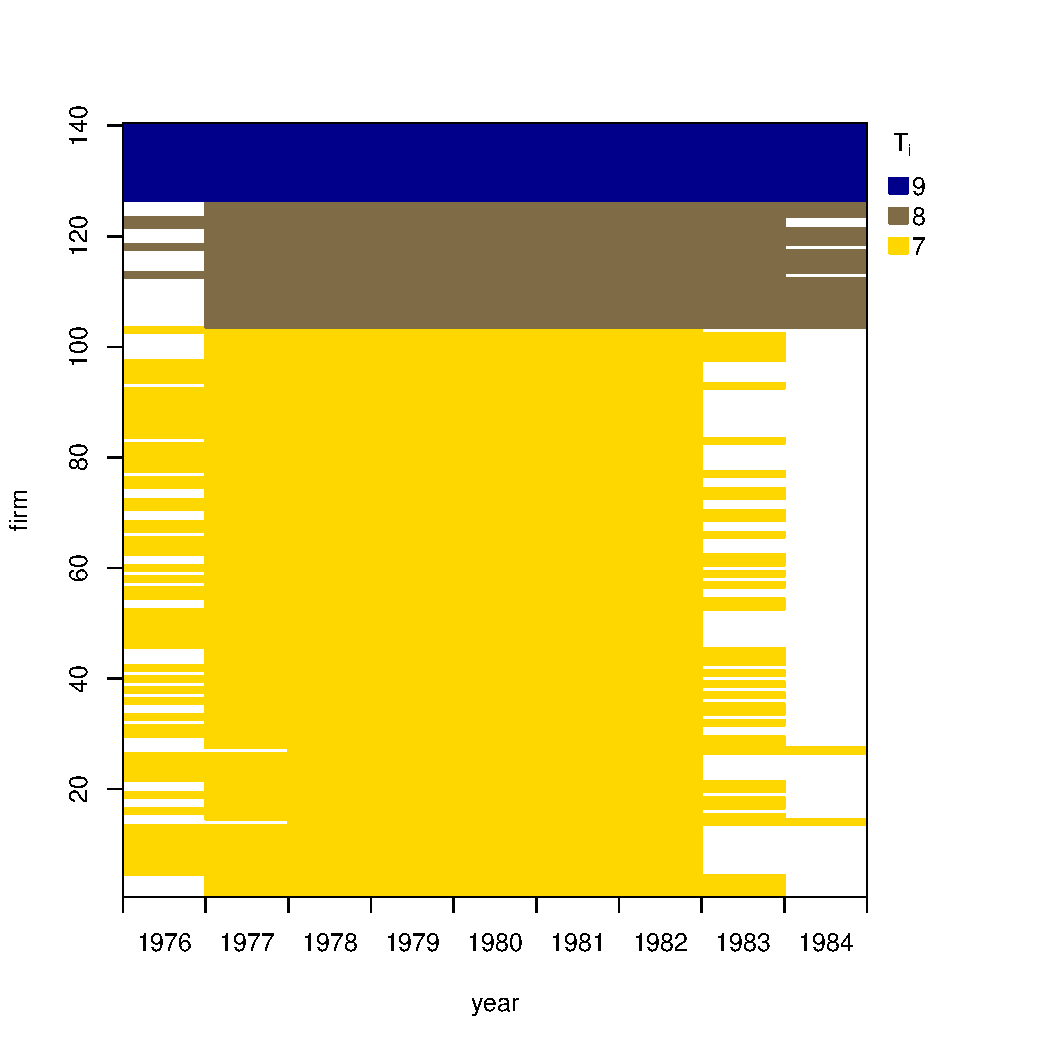
\includegraphics[width = 8cm, height = 8cm]{strucUPD_plot.pdf}
  \caption{Unbalanced panel structure plot.}\label{fig:strucUPDplot}
\end{figure}
Figure \ref{fig:strucUPDplot} indicates the time periods (compare abscissa) available for each cross-sectional unit (ordinate). Blank areas represent missing observations. The coloring scheme shows the number of time series units that are available for the corresponding cross-sectional units. We see that the given dataset has already been ordered by the number of time periods available.









The goal of the empirical analysis is to estimate the lag parameters $\alpha_1$ and $\alpha_2$ and the coefficients $\beta_j$ of the $j=1, \dots, 8$ further covariates while controlling for (unobserved) time effects and accounting for unobserved individual-specific heterogeneity. In the following, we first apply \pkg{pdynmc} to replicate the original results of \citet{AreBon1991} that are based on HNR moment conditions only and introduce the implemented tests. Then, we provide results for adding ABov moment conditions to the analysis. Finally, we discuss results for HNR moment conditions extended by AS moment conditions and apply iterated GMM. All results on estimated coefficients and robust standard errors are summarized in Table \ref{Tab01:estimates}. Details on employed moment conditions are provided in the table footnotes.

\begin{table}[hptb]
\begin{tabular}{lccccc}
  \hline

                & (a)           & (b)           & (c)           & (d)           & (e)           \\
                & 1-Step Estimate      & 2-S.\ Estimate      & 2-S.\ Estimate      & 2-S.\ Estimate      & Iterated Est.\      \\
                & HNR only      & HNR only      & HNR \& ABov   & HNR \& AS     & HNR \& AS      \\
                & (SE Rob.)     & (SE Rob.)     & (SE Rob.)     & (SE Rob.)     & (SE Rob.)     \\
  \hline
  L1.n  & 0.686{***}      & 0.629{**}       & 1.103{***}      & 1.112{***}      & 1.197{***}           \\
        & (0.145)         & (0.193)         & (0.050)         & (0.066)         & (0.069)              \\
  L2.n  & -0.085          & -0.065          & -0.104{*}       & -0.071          & -0.126               \\
        & (0.056)         & (0.045)         & (0.047)         & (0.069)         & (0.068)              \\
  w     & -0.608{***}     & -0.526{***}     & -0.448{**}      & -0.417{**}      & -0.219               \\
        & (0.178)         & (0.155)         & (0.149)         & (0.153)         & (0.127)              \\
  L1.w  & 0.393{*}        & 0.311           & 0.423{**}       & 0.413{**}       & 0.258                \\
        & (0.168)         & (0.203)         & (0.156)         & (0.160)         & (0.138)              \\
  k     & 0.357{***}      & 0.278{***}      & 0.290{***}      & 0.309{***}      & 0.255{***}           \\
        & (0.059)         & (0.073)         & (0.050)         & (0.053)         & (0.056)              \\
  L1.k  & -0.058          & 0.014           & -0.153{*}       & -0.189{**}      & -0.155{*}            \\
        & (0.073)         & (0.092)         & (0.067)         & (0.068)         & (0.077)              \\
  L2.k  & -0.020          & -0.040          & -0.137{***}     & -0.154{**}      & -0.156{**}           \\
        & (0.033)         & (0.043)         & (0.041)         & (0.050)         & (0.055)              \\
  ys    & 0.609{***}      & 0.592{***}      & 0.548{**}       & 0.582{**}       & 0.530{**}            \\
        & (0.173)         & (0.173)         & (0.194)         & (0.178)         & (0.183)              \\
  L1.ys & -0.711{**}      & -0.566{*}       & -0.666{**}      & -0.624{**}      & -0.379               \\
        & (0.232)         & (0.261)         & (0.221)         & (0.216)         & (0.223)              \\
  L2.ys & 0.106           & 0.101           & 0.127           & 0.023           & -0.208               \\
        & (0.141)         & (0.161)         & (0.156)         & (0.151)         & (0.152)              \\
  1979  & 0.010           & 0.011           & 0.024{*}        & 0.027{*}        & 0.031{**}            \\
        & (0.010)         & (0.012)         & (0.011)         & (0.011)         & (0.010)              \\
  1980  & 0.022           & 0.023           & 0.041{*}        & 0.047{**}       & 0.053{**}            \\
        & (0.018)         & (0.020)         & (0.020)         & (0.018)         & (0.018)              \\
  1981  & -0.012          & -0.021          & 0.002           & 0.018           & 0.026                \\
        & (0.030)         & (0.033)         & (0.034)         & (0.030)         & (0.030)              \\
  1982  & -0.027          & -0.031          & 0.018           & 0.022           & 0.034                \\
        & (0.029)         & (0.034)         & (0.023)         & (0.021)         & (0.023)              \\
  1983  & -0.021          & -0.018          & 0.043{*}        & 0.037{*}        & 0.041{*}             \\
        & (0.030)         & (0.037)         & (0.018)         & (0.019)         & (0.021)              \\
  1984  & -0.008          & -0.023          & 0.029           & 0.015           & 0.021                \\
        & (0.031)         & (0.037)         & (0.022)         & (0.022)         & (0.024)              \\
   \hline
    \multicolumn{6}{l}{\scriptsize{}(a, b) Equations in differences: \phantom{le}$L\left(2/8\right).n,D.w,L.D.w,D.k,L.D.k,L2.D.k,D.ys,L.D.ys,L2.D.ys,D.1979-D.1984$} \\
    \multicolumn{6}{l}{\scriptsize{}(c)\phantom{, b} Equations in differences: \phantom{le}$L\left(2/8\right).n,D.w,L.D.w,L2.D.w,D.k,L.D.k,L2.D.k,D.ys,L.D.ys,L2.D.ys,D.1979-D.1984$} \\
    \multicolumn{6}{l}{\scriptsize{}\phantom{(c, b)} Equations in levels: \phantom{encesee}$L\left(1/7\right).D.n,w,L.w,L2.w,k,L.k,L2.k,ys,L.ys,L2.ys$} \\
    \multicolumn{6}{l}{\scriptsize{}(d, e) Equations in differences: \phantom{le}$L\left(2/8\right).n, u ,D.w,L.D.w,L2.D.w,D.k,L.D.k,L2.D.k,D.ys,L.D.ys,L2.D.ys,D.1979-D.1984$} \\
    \multicolumn{6}{l}{\scriptsize{}\phantom{(d, b)} Equations in levels: \phantom{encesee}$w,L.w,L2.w,k,L.k,L2.k,ys,L.ys,L2.ys$} \\
    \multicolumn{6}{l}{\scriptsize{}{*} $p<0.05$, {**} $p<0.01$, {***} $p<0.001$ (refers to $t$-test of the null that the coefficient is equal to zero)} \\
\end{tabular}
\centering\caption{Estimates in the spirit of Table 4 in \citet{AreBon1991}. Use of $L(a_1/a_2)$ indicates lag transformation by a minimum of $a_1$ and a maximum of $a_2$ time periods; $D$ indicates first differences. Table footnotes indicate available instruments and corresponding equations.} \label{Tab01:estimates}
\end{table}

















\subsection{GMM estimation with HNR moment conditions} \label{sec:HNRmcEstimation}
When reproducing the results in Table 4 on p. 290 of \citet{AreBon1991} with \pkg{pdynmc}, the model structure underlying Equation (\ref{EQ18:ABEstimation}) can be specified and estimated by:
\begin{example}
m1 <- pdynmc(
  dat = dat, varname.i = "firm", varname.t = "year",
  use.mc.diff = TRUE, use.mc.lev = FALSE, use.mc.nonlin = FALSE,
  include.y = TRUE, varname.y = "n", lagTerms.y = 2,
  fur.con = TRUE, fur.con.diff = TRUE, fur.con.lev = FALSE,
  varname.reg.fur = c("w", "k", "ys"), lagTerms.reg.fur = c(1,2,2),
  include.dum = TRUE, dum.diff = TRUE, dum.lev = FALSE, varname.dum = "year",
  w.mat = "iid.err", std.err = "corrected",
  estimation = "onestep", opt.meth = "none"
)
\end{example}
The standard output is accessed via \code{summary(m1)} and can be found in panel (a) of Table \ref{Tab01:estimates}.
The estimated coefficients reproduce the estimates in Table 4, column (a1) on p. 290 of \citet{AreBon1991} when one specifies all arguments as stated in this section.
Changing the argument \code{estimation} to \code{twostep} yields two-step GMM coefficient estimates (the \code{pdynmc}-output object is assigned to \code{m2}) from Table 4, column (a2) on p. 290 of \citet{AreBon1991}. These results may be found in panel (b) of Table \ref{Tab01:estimates}.
Note that the standard errors presented in column (b) of Table \ref{Tab01:estimates} are based on the Windmeijer-correction and deviate from the conventional standard errors reported in \citet{AreBon1991}. Standard errors from the original analysis can be reproduced by setting \code{std.err = "unadjusted"}.


The command \code{mtest.fct(m2, t.order = 2)} is used to perform the test of \citet{AreBon1991} for second order serial correlation and yields:
\begin{example}
        Arellano and Bond (1991) serial correlation test of degree 2

data:  2step GMM Estimation; H0: no serial correlation of order 2 in the error terms
normal = -0.37133, p-value = 0.7104
\end{example}
The test does not reject the null hypothesis at any plausible significance level and provides no indication that the model specification might be inadequate.

Computing the Hansen $J$-test of overidentifying restrictions by \code{jtest.fct(m2)} yields:
\begin{example}
        J-Test of Hansen

data:  2step GMM Estimation; H0: overidentifying restrictions valid
chisq = 31.381, df = 25, p-value = 0.1767
\end{example}
As the test does not reject the null hypothesis, there are no indications that the validity of the instruments (i.e., the model assumptions) employed in estimation may be in doubt.

For the Wald test of the null hypothesis that the population parameters of all coefficients included in the model are jointly zero, which is tested by \code{wald.fct(m2, param = "all")}, we obtain:
\begin{example}
        Wald test

data:  2step GMM Estimation; H0: all parameters are jointly zero
chisq = 1100, df = 16, p-value < 2.2e-16
\end{example}
The test rejects the null hypothesis.
Hence, all tests shown here provide no indications that the model in column (b) of Table \ref{Tab01:estimates} is misspecified.



Comparing the results to xtabond2 shows that degrees of freedom and $p$-values differ for the latter two tests. We consider 25 degrees of freedom to be the appropriate number in the J-test, as 41 instruments are employed in estimation to obtain 16 coefficient estimates. The latter number (16) is the appropriate number of degrees of freedom in the Wald test. It seems that the function xtabond2 does not correct the degrees of freedom for the number of dummies dropped in estimation\footnote{Dummies are dropped by the estimation routine in case of high collinearity.}. The difference in the $p$-value is due to the differences in the degrees of freedom. Our results are equivalent to the results of \code{pgmm} for the overidentifying restrictions test (referred to as ``Sargan test'' in \code{pgmm}).

Using many instruments may have undesirable side effects such as biased coefficient estimates and standard errors. This may result in misleading inference and specification tests \citep[see, e.g.,][]{Roo2009}. The number of lags of the dependent variable which are used to derive moment conditions can be limited by setting \code{maxLags.y} (equivalently lags of, for example, endogenous covariates can be limited via \code{maxLags.reg.end}). Setting \code{maxLags.y = 4} reduces the number of HNR moment conditions for the GMM estimation above from 27 to 17 and the total number of instruments employed in the estimation from 41 to 31.









\subsection{GMM estimation with HNR and ABov moment conditions} \label{sec:HNRABmcEstimation}
When the ``constant correlated effects'' assumption stated in Equation (\ref{EQ07:CCE}) holds, the HNR moment conditions from equations in differences employed in Section \hyperref[sec:HNRmcEstimation]{GMM estimation with HNR moment conditions} can be extended by the ABov moment conditions from equations in levels.

The ABov moment conditions are particularly useful for data generating processes, which are highly persistent \citep{BluBon1998}. In this case, identification by the HNR moment conditions from equations in differences may fail, and GMM estimation based on HNR moment conditions is documented to possess poor finite sample performance \citep[see, e.g.,][]{BluBon1998,BluBonWin2001,BunSar2015}.

In \pkg{pdynmc}, the ABov moment conditions from equations in levels can be (additionally) incorporated by:
\begin{example}
use.mc.lev = TRUE
\end{example}
In principle, both time dummies and further covariates can be included in the equations in first differences and the level equations. It is recommended, though, to include the dummies only in one of the equations, as it can be shown that incorporating them in both equations renders one set of dummies redundant for estimation -- while for non-lagged dependent covariates, this equivalence does not hold.\footnote{Note that this is the case in balanced panels. The results may also not be numerically identical across function calls for different choices of the one-step weighting matrix. For a discussion, see \url{https://www.statalist.org/forums/forum/general-stata-discussion/general/1357268-system-gmm-time-dummies}.} We accommodate non-lagged dependent covariates in the levels equations by:
\begin{example}
fur.con.lev = TRUE
\end{example}
for all subsequent estimations of this example.
The results presented in column (c) of Table \ref{Tab01:estimates} are two-step estimates of column (a2) of Table 4 in \citet{AreBon1991} extended by ABov moment conditions.

Including ABov moment conditions into the analysis leads to substantial changes in the coefficient estimates of the first lag of the dependent variable. Note that the results indicate a markedly higher persistence of employment and render including two lags of the dependent variable questionable \citep[][e.g., estimate a version of the equation which contains only one lag of all covariates]{BluBon1998}. Note that the coefficient estimates of the covariates, besides the first lag of the dependent variable, appear to be similar across estimations.


Equivalent results to column (c) of Table \ref{Tab01:estimates} can be obtained from the \code{pgmm} function in the \pkg{plm}-package. When replicating the results with xtabond2, \code{inst.stata = TRUE} in \pkg{pdynmc} ensures that results are equivalent.








\subsection{GMM estimation with HNR and AS moment conditions}
Recall that the linear ABov moment conditions from equations in levels encompass the nonlinear AS moment conditions (\citealp[][]{BluBon1998}; \citealp[a derivation is provided in][]{Fri2019}). Both sets of moment conditions may be useful in GMM estimation when the lag parameter is close to unity, and it can be shown that extending the HNR moment conditions by either the ABov or the AS moment conditions may identify the lag parameter -- even when individual moment conditions fail to do so \citep{BluBon1998,BunKle2014,GorHanXue2016}. The ABov moment conditions require the ``constant correlated effects'' assumption to hold, while the AS moment conditions only require standard assumptions to hold. Therefore, the latter may be useful in situations where the ``constant correlated effects'' assumption is in doubt, and the statistician aims to investigate a highly persistent dynamic process with a structure similar to Equation (\ref{EQ01:lin-dyn-pdm}).
In \pkg{pdynmc}, including nonlinear moment conditions into the analysis is available via:
\begin{example}
use.mc.nonlin = TRUE
\end{example}
When extending the analysis of \citet{AreBon1991} by the nonlinear AS moment conditions, the results differ substantially from column (b) of Table \ref{Tab01:estimates} and are very similar to the coefficient estimates shown in column (c) of Table \ref{Tab01:estimates}. This indicates high persistence in the employment process that leads to lag parameters not being identified by the HNR moment conditions \citep{BunKle2014,GorHanXue2016}.

Additionally, we employ iterated GMM via:
\begin{example}
estimation = "iterative", max.iter = 100, iter.tol = 0.01,
\end{example}
Iterated GMM results are shown in column (e) of Table \ref{Tab01:estimates}. The moment conditions employed are the same as in column (d) of the table. The parameter estimates obtained after 13 steps are relatively similar to those in columns (c)-(d). The ranges of the coefficient estimates across GMM iterations are displayed in Figure \ref{fig:pdynmc_coef_range}. This plot is available for two-step and iterated GMM estimates via command \code{plot(m5, type = "coef.range", omit1step = TRUE)}. Using command \code{plot(m5)} yields a scatterplot of fitted values and residuals of a fitted model object, instead.
%and is also available for one-step estimates.

\begin{figure}[ht]
  \centering
  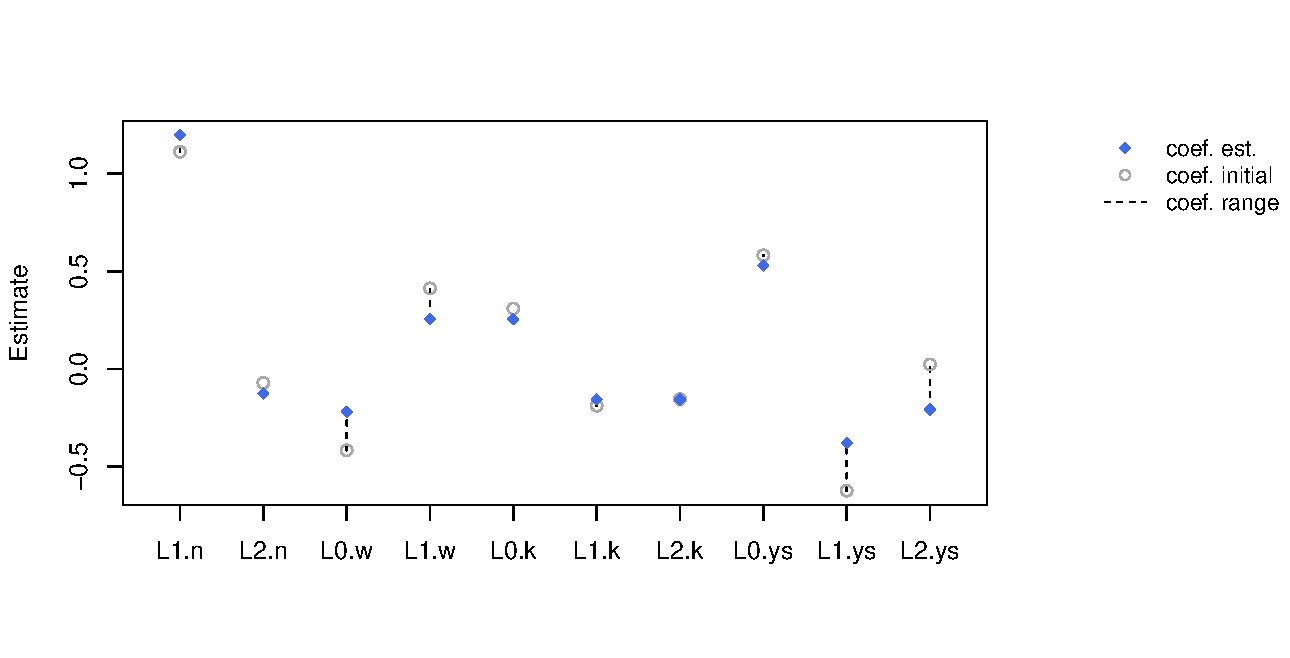
\includegraphics[width = 12cm, height = 6cm]{plot_pdynmc_coef_range.pdf}
  \caption{Estimated coefficients and corresponding coefficient ranges during iterated GMM estimation (ordinate) for the covariates (dummy variables excluded). Coefficient estimates at the initial step are displayed as grey open circles and the estimates at the last step as blue diamonds.}\label{fig:pdynmc_coef_range}
\end{figure}

Figure \ref{fig:pdynmc_coef_range} indicates coefficient estimates at iteration 2 as grey open circles (the first iteration is ignored due to \code{omit1step = TRUE}) and estimates at the last iteration as blue diamonds. For the estimates displayed in column (e) of Table \ref{Tab01:estimates}, we observe that the lag parameters are relatively stable across iterations and resemble the two-step estimates; for the further covariates, larger changes in coefficient estimates across iterations occur for coefficients with larger standard errors (compare $w$, $k$, and $ys$).

As an additional tool to investigate coefficient estimates from iterated GMM, coefficient path plots \citep[compare][Figure 1]{HansenLee2020} are provided. Figure \ref{fig:pdynmc_coef_path} illustrates the path of coefficient estimates for lag parameter $\alpha_1$ across GMM iterations and is obtained via \code{plot(m5, type = "coef.path", co = "L1.n")}. Argument \code{co} allows to draw the path(s) of particular coefficient estimates; per default, all coefficients (apart from time dummies) are included in the plot. Approximate 95\% confidence bands were added to the plot for the final iteration (available by setting argument \code{add.se.approx = TRUE}).
\begin{figure}[ht]
  \centering
  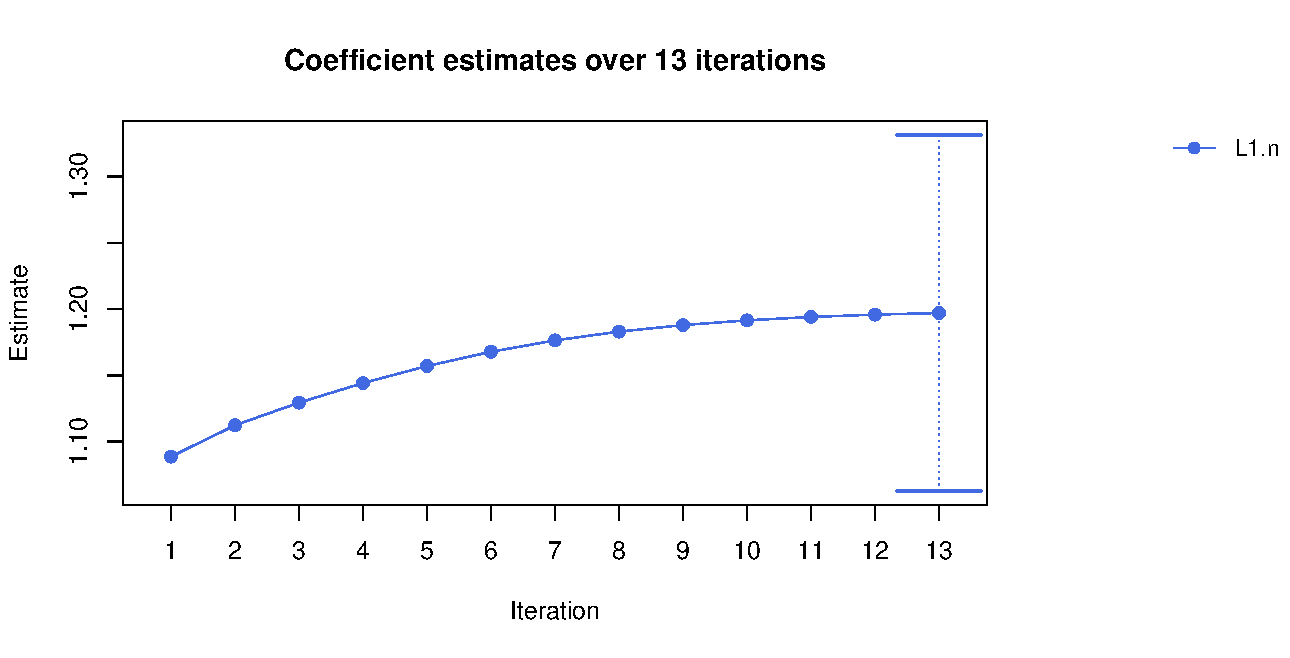
\includegraphics[width = 12cm, height = 6cm]{plot_pdynmc_coef_path.pdf}
  \caption{Estimated coefficient path for lag parameter $\alpha_1$ during iterated GMM estimation and corresponding approximate 95\% confidence bands for final iteration.}\label{fig:pdynmc_coef_path}
\end{figure}


Overall, the results displayed in columns (c)-(e) of Table \ref{Tab01:estimates} suggest that the employment process may be highly persistent and that using only HNR moment conditions may not be sufficient to identify the parameters.
In practice, contrasting GMM estimates based on HNR and AS moment conditions with GMM estimates based on HNR and ABov moment conditions can be used as a robustness check of the ``constant correlated effects'' assumption: When estimates differ, this may cast doubt on the assumption. Here, this is not the case as the results in column (c) are very close to those in (d) and (e).















\section{Conclusion} \label{sec:conclusion}

R-package \pkg{pdynmc} provides a function to estimate linear dynamic panel data models based on linear and nonlinear moment conditions. The implementation reflects recent developments in the literature by including iterated GMM and offers a wide variety of configuration options.
The package provides the only open source solution for GMM estimation of dynamic panels with linear and nonlinear moment conditions, aligns commercial and non-commercial software, and is implemented to enable the user to exert precise control over all functionality. Additionally, suitable visualizations of panel data structures and ranges and paths of coefficient estimates across GMM iterations are provided.

The functionality of \pkg{pdynmc} includes that it allows for general lag structures of the covariates; further controls and external instruments (if available) may also be added. The estimation routine can handle balanced and unbalanced panel datasets and provides one-step-, two-step-, and iterated estimation. Accounting for (unobserved) time-specific effects is possible by including time dummies.
Estimation relies on numerical optimization of the GMM objective function. Corresponding closed-form solutions are computed -- where possible -- and stored beside the results from numerical optimization.
Different choices for the weighting matrix, which guides the aggregation of moment conditions in one-step GMM estimation are available.
Robust standard errors are available for inference and specification testing. Nonlinear moment conditions provide a robustness check of the frequently employed constant correlated effects assumption.






\section{Acknowledgements}
We thank the executive editor and anonymous reviewers for their helpful comments and suggestions.
We also thank Harry Haupt for helpful discussions, comments, and suggestions.
Andrew Adrian Pua is supported by the Fundamental Research Funds for the Central Universities (20720171074), the Basic Scientific Center Project 71988101 of National Science Foundation of China, and the 111 Project (B13028).






\bibliography{fritsch-pua-schnurbus}

\address{Markus Fritsch\\
  University of Passau\\
  School of Business, Economics, and Information Systems\\
  94032 Passau\\
  Germany\\
  \email{markus.fritsch@uni-passau.de}}

\address{Andrew Adrian Yu Pua\\
  MOE Key Laboratory of Econometrics\\
  The Wang Yanan Institute for Studies in Economics\\
  Department of Statistics, School of Economics\\
  Fujian Key Laboratory of Statistics\\
  Xiamen University\\
  China\\
  \email{andrewypua@outlook.com}}

\address{Joachim Schnurbus\\
  University of Passau\\
  School of Business, Economics, and Information Systems\\
  94032 Passau\\
  Germany\\
  \email{joachim.schnurbus@uni-passau.de}}











